\documentclass[]{final_report}
\usepackage{graphicx}
\graphicspath{ {./images/}{../../media/images} }
\usepackage{hyperref}
\usepackage{amssymb}
\usepackage{amsmath}
\usepackage{dirtytalk}
\usepackage{calligra}
\usepackage{subcaption}
\usepackage{float}
\providecommand{\tightlist}{%
  \setlength{\itemsep}{0pt}\setlength{\parskip}{0pt}}

%%%%%%%%%%%%%%%%%%%%%%
%%% Input project details
\def\studentname{Cougar Tasker}
\def\reportyear{2023-24}
\def\projecttitle{Resourceful Robots}
\def\supervisorname{Dr. Anand Subramoney}
\def\degree{MSci (Hons) in Computer Science (Artificial Intelligence)}
\def\fullOrHalfUnit{Full Unit} % indicate if you are doing the project as a Full Unit or Half Unit
\def\finalOrInterim{Final Report} % indicate if this document is your Final Report or Interim Report

\begin{document}

\maketitle

%%%%%%%%%%%%%%%%%%%%%%
%%% Declaration

\chapter*{Declaration}

This report has been prepared on the basis of my own work. Where other published and unpublished source materials have been used, these have been acknowledged.

\vskip3em

Word Count: 

\vskip3em

Student Name: \studentname

\vskip3em

Date of Submission: 08/12/2023

\vskip3em

Signature: {\calligra \LARGE \studentname}

\newpage

%%%%%%%%%%%%%%%%%%%%%%
%%% Table of Contents
\tableofcontents\pdfbookmark[0]{Table of Contents}{toc}\newpage

%%%%%%%%%%%%%%%%%%%%%%
%%% Your Abstract here

\begin{abstract}

  \section{TODO - (Rework Rationale) Resourceful robots}
  
  To complete many objectives robotic agents need to adapt and learn new environments. This presents a problem for traditional supervised learning approaches that operate under the (IID) assumption\cite{bagnell2005robust}, training data may not apply to new environments. This report investigates reinforcement learning (RL) techniques as an alternative for this class of robotics. Reinforcement Learning is a machine-learning paradigm where the learning component receives external judgment like supervised learning. However, in reinforcement learning this judgment is provided after the agent decides on the consequences of their actions. this is unlike supervised learning; there is no need for training in RL the agent will continuously learn from their successes and failures. Although RL does not need training data it is also unlike unsupervised learning, since RL agents learn to achieve more reward from within the system rather than observing underlying patterns.
  
  These unique benefits of reinforcement learning make this field applicable to many real-world problems. RL is built upon a strong mathematical foundation that allows us to make strong guarantees about solutions in the reinforcement learning domain. Furthermore, RL spans widely uniting together many important and diverse areas of study such as Economics, Optimisation, Game Theory, robotics and Cognitive Science.
  
  It follows that the primary goal of this project is to understand and implement reinforcement learning. As this project develops the secondary aim is to frame these solutions from the perspective of autonomous robotic agents to aid in decision-making. This robotics background fits well with this project's other requirements: such as implementing a grid world environment and Q-learning agents. Resource-gathering robots from autonomous vacuum cleaners to industrial warehouse robots can be modelled in these grid world environments and this project aims to create reinforcement learning agents that are successful in these environments. Although the project is not limited to these technologies we will also evaluate more advanced techniques such as deep reinforcement learning agents and diverse RL environments from the gymnasium library.
  
\end{abstract}

%%%%%%%%%%%%%%%%%%%%%%
%%% Introduction 

\chapter{TODO - Introduction}




\section{TODO (rework + extend) - Aims and Objectives}
\begin{itemize}
  \item Efficient Navigation: The agent must autonomously navigate a grid world while making decisions to optimise rewards. The robot should learn to prioritise efficient paths.
  \item Balancing Constraints: The agent must balance collecting resources with constraints such as energy expenditure. The robot should adapt its behaviour based on the availability of resources and its current energy levels.
  \item General Approach: The agent must not use any environment-specific techniques. It should learn from and function in any Markov environment.
  \item Deep Reinforcement Learning: The program should integrate deep neural networks (DNN) with Q-learning.
  \item Visualisation: The program should provide a GUI that visualises the operation of these agents interactively.
\end{itemize}

\section{Motivation}

My inspiration for studying for this degree, specialising in artificial intelligence, comes in large part from my belief that AI is becoming increasingly pivotal in shaping the future of technology and industry. For this purpose, this project presents an invaluable opportunity for my personal and professional growth. It is a fantastic platform to improve my comprehension of reinforcement learning while offering hands-on experience. 

What is unique about this resource-gathering robot project is its structured progression of complexity, Starting from fundamental concepts and culminating in advanced techniques. This gradient makes the complex nature of reinforcement learning more approachable than it may be in industry. 

This project interests me because of its generality and applicability to many different scenarios. Resource-gathering has the potential to incorporate many real-world constraints like energy, visibility and obstacles. I would like to see how this impacts different exploration strategies.

Last year, I completed my year-long internship at Zing Dev (Zing), a digital communications company that is progressively incorporating AI systems for its customers. This experience has demonstrated to me the value of understanding the internals of these AI systems. It is clear that AI is a clear focus for most companies, Ransbotham et al. said: 
\begin{quote}
  Almost 85\% believe AI will allow their companies to obtain or sustain a competitive advantage \cite{ransbotham2017reshaping}
\end{quote}

Through this project, I aim to improve my understanding of autonomous agents' benefits, biases, and limitations. This knowledge will be desirable for many companies like Zing working with artificial agents.


\section{TODO - Literature Review}


Full critical review of literature relevant to the study.


\chapter{TODO (section introduction)- Software Engineering}

\begin{figure}[H]
  \centering
  \begin{subfigure}{.5\textwidth}
    \centering
    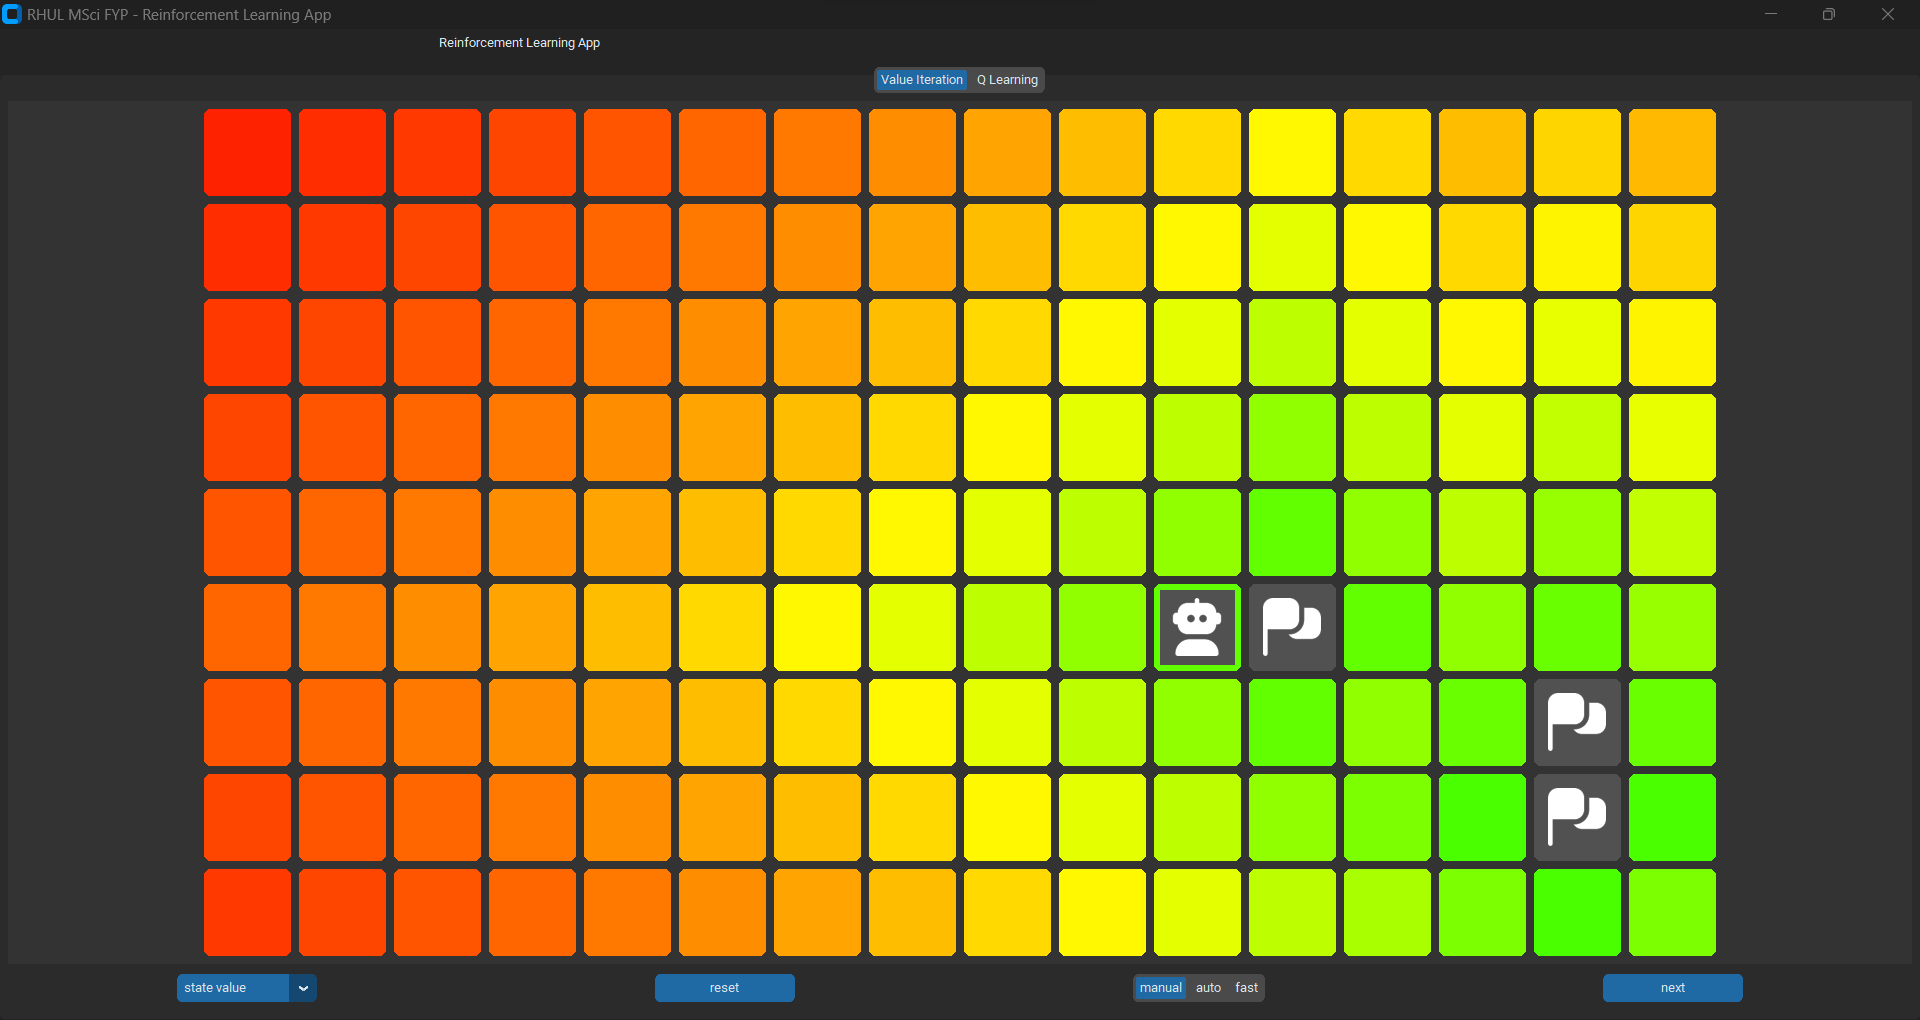
\includegraphics[width=0.95\linewidth]{state_value}
    \caption[width=0.5\linewidth]{\label{fig:screenshot:state-value-table} The V (state-value) table}
  \end{subfigure}%
  \begin{subfigure}{.5\textwidth}
    \centering
    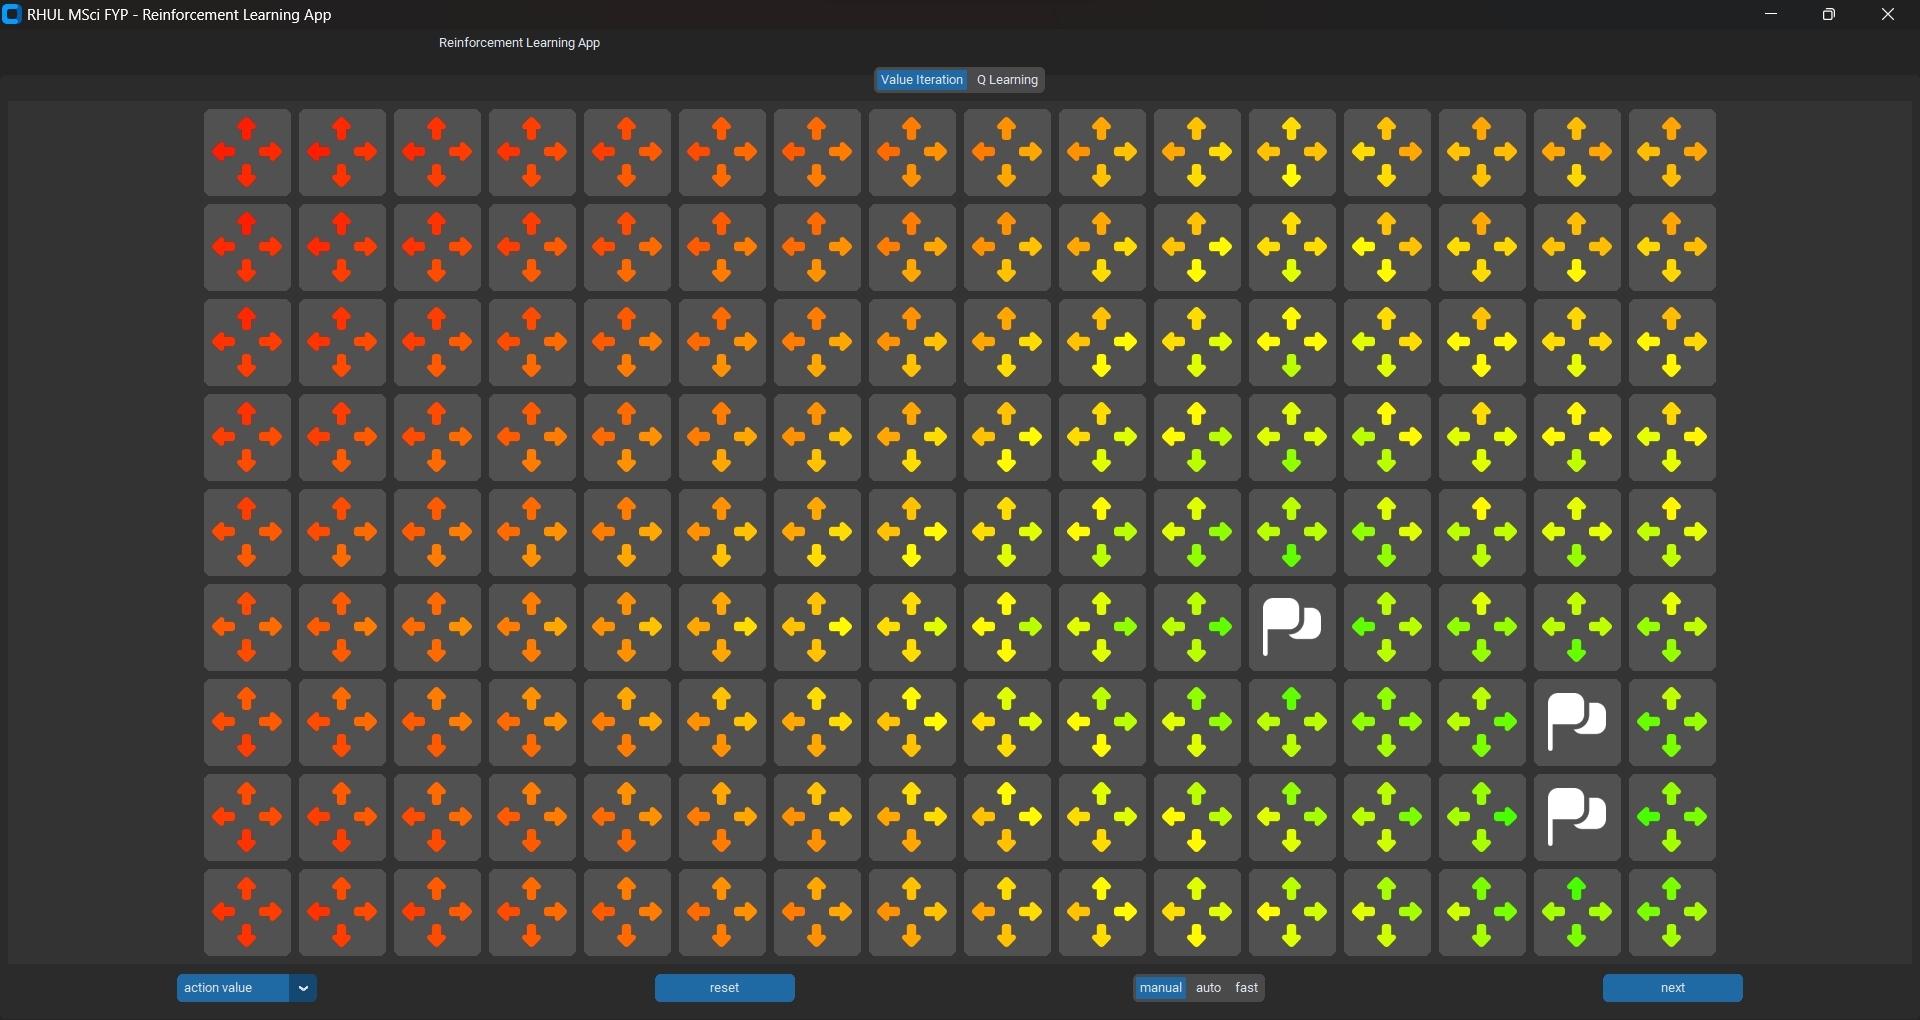
\includegraphics[width=0.95\linewidth]{action_value}
    \caption[width=0.5\linewidth]{\label{fig:screenshot:action-value-table} The Q (action-value) table}
  \end{subfigure}
  \caption{Two of the application's visualisations}
  \label{fig:app-ui}
\end{figure}

This chapter details the software engineering of the project and demonstrates how this allowed the project to succeed. Software engineering consists of methods and techniques to develop large and robust applications\cite{van2008software}.  

\section{System Design}


This application has been written in Python with the model-view-controller architecture. Python was chosen for many reasons such as it has a strong ecosystem of machine learning libraries that are crucial for performant deep reinforcement learning. Python is also a high-level language that is clear and readable. However, python has notable constraints.  The predominant Python interpreter, CPython, is substantially slower than other implementations\cite{pythonMachineLearning}. For compatibility, I have chosen this interpreter. To mitigate the effects in the most performance-sensitive areas of the application I have used libraries such as Numpy, Numba and Pillow that allow me to move the bulk of the computation out of Python.  

The application has a complex GUI with controls that visualise the state of more complex reinforcement models. The model-view-controller architecture is well suited for this application's requirements it helps to reduce the coupling between these two different but connected modules. This has proved invaluable several times as I needed to change the GUI library several times to meet my requirements. Due to the nature of modern GUI frameworks, the code traditionally considered the view receives update signals from the user. For this reason, this project requires the use of the layered MVC pattern \cite{webMVC}\cite{gamesMVC} where the controller acts as a bridge between the model and view. 

The application has been written in an object-oriented fashion with modern software engineering principles in mind\cite{van2008software}. Object-oriented code is a programming paradigm built around the idea of combining state and functionality into one entity called an object. The goal of object-oriented code in this project and software engineering is to reduce coupling and increase cohesion. Coupling describes how interrelated different objects are while cohesion describes how related code is within the same object. In this application this is achieved by adhering to software engineering principles \cite{softwareEngineringPrinciples} and using software design patterns where applicable.

\section{TODO - Technical Decisions}


 - multiprocessing architecture the use of IPC + serialization

talk about the choice of gui,  , etc.

Are important (technical) decisions well made and **argued**? This includes:

 - good design decisions
 - choice or development of algorithms
 - scope of the project.



\pagebreak
\section{Workflow}


All aspects of this project are stored under the Git version control system, and changes made on this project are grouped into small units called commits. Each commit belongs to a branch and has a message summarising the changes. Conventional commits \cite{conventionalCommitsOnline} is a standard for commit messages. In this project, I have followed this standard because it keeps the commit message consistent and enables the use of tools such as automated change log generation and versioning. As this project has a single author I have chosen to use branches to group together related work, instead of following a specific branching strategy. However, like most branching strategies the main branch represents the project after each stage of work is finalised and therefore main is always is complete and functional. 

One key part of this project and its workflow is documentation. The documentation is written alongside the code in what are called docstrings. This serves many purposes firstly the co-location helps keep the documentation in sync with the application. Special linting rules ensure that these docstrings are written consistently for every piece of code ensuring 100\% documentation coverage. Docstrings are also integrated into the Python language with the `help` command and most editors also integrate docstrings so they are accessible during development. Importantly this documentation is made accessible as a documentation site. This site is generated automatically for these docstrings and other aspects of the code. This process results in a searchable, linked documentation page that is up-to-date\cite{pythonAutoDoc} and covers all of the code. 

Testing is integral to this project, as part of my workflow I write unit tests. Unit tests are pieces of code that perform validation and verification parts of the main application. A unit testing framework has been configured to run these tests and collate the results. All tests must pass before each commit can be made this means that regressions are spotted quickly. These tests are also integrated into the IDE providing feedback and easing debugging.  While testing can be valuable it can be costly, Daka et al found developers spent a substantial time writing tests \cite{unitTestingSurvey}. The returns from testing can be especially low for trivial code that can take several times longer to test than create. For this reason I have limited tests to all important areas or complex areas of the program.  

The development environment is the system of programs where this workflow takes place. This project is configured to work well with a particular Integrated development environment (IDE), for instance, the IDE will be able to start the application with a debugger attached allowing the user to step through the code in the editor. Code quality is maintained in this repository with several automated tools. Static code analysis tools enforce a consistent code style and check for typing errors. I have configured these tools to integrate with the IDE giving immediate feedback so issues can be addressed quickly. Furthermore, Git is configured with pre-commit hooks so these tools must run and validate the code before every commit is made. Furthermore, these tools can be integrated with CI/CD pipelines which is particularly useful for collaborative projects.

While all of the tooling for this project improves many aspects of development this may be difficult to set up and provides many opportunities for discrepancies to emerge between different setups. For this reason, I have created a development container, This container fully specifies every tool and its version to be installed. This containerised environment makes it easy to set up the environment and consistent each time. Containers for development are rapidly growing in interest\cite{developmentContainers}. 

For the sake of consistency, the application itself has been configured with a dependency management and packaging tool. All of the libraries the application relies upon are specified in the standard `pyproject.toml` and the tool manages their installation in an isolated virtual environment. This process makes it easy to distribute this application and avoids inconsistencies on different computers.

\section{Functionality and Usage}

The application's functionality revolves around running reinforcement learning simulations and allowing the user to interact with and analyse the effects of different options. These simulations encompass two main units an agent and dynamics. The agent unit encompasses the functionality for learning and decision making while the dynamics unit encompasses a grid world Markov decision process. These units are interchangeable and configurable by the user dynamically through controls in the user interface and through a configuration file \path{config.toml}. The results of these learning experiments are expressed by the application in several fashions such as a state-by-state view, information displays and graphs.


\subsection{Getting Started}

The project is set up as a standard distribution package, poetry is the build backend. While you may also use poetry as the build front-end if you have it installed however it may be excessive if you are only interested in starting the application.

Pipx is a simple build frontend that should be familiar if you have experience with pip. You can find instructions on how to \href{https://pipx.pypa.io/stable/installation/}{install Pipx for your platform here}. If you have installed pipx you can run the application with the following command:

\begin{verbatim*}
  python3 -m pipx run --spec . start
\end{verbatim*}

You can find more information about this application and how to start it in the readme file in the code folder.

\section{User Interface}

The user interface is not only a major component of the project's functionality but also the user's window into the entire application. When starting the application you will be greeted by a window that is largely broken into three components. At the top, there is a section which contains the main controls for selecting the most significant options of the main simulation; such as the agent and dynamics. If the agent is off-policy you can select its exploration strategy. 

In the middle, there is a tabbed area the first tab is the main display this section visualises the state of the main simulation. The second tab displays the reward history of the simulation as a graph. The third and fourth tabs can run auxiliary simulations in the background to examine the effect of different hyperparameter choices. The third tab shows graphs of the effects of varying each hyperparameter and the reward achieved with 95\% confidence bounds. Finally, the fourth tab controls a random search procedure, starting this procedure searches for the best parameter choices for minimising regret. All of the graphs allow you to save their contents to a file of your choosing. 

The main display on the first tab visualises the current state of the main simulation, each dynamics are based around a grid world and the display visualises this with a grid of cells, each cell representing a possible position the agent can occupy. The function of this grid will vary based on the display mode, In the initial default display mode a robot icon represents the agent's location, flags represent the agent's goals and stop icons represent obstacles. In other Display modes arrows represent the agent's actions in each state and a color scale is used to represent the agent's interpretation of value. On this color scale hues vary from red to green, where red is the least valuable state and green is the most valuable state or state-action.

At the bottom are specific controls specific to the main simulation and its visualisation. For example, there are controls for selecting the display mode and allowing the user to step through the simulation manually or automatically. 

\chapter{Professional Issues In Machine Learning}

Machine learning programs and techniques, as explored in this project, possess immense potential for social benefit when managed judiciously, but they also risk significant social and ethical consequences\cite{AISocialImpactAndAccountability}. One concern is the ability of ML systems to reinforce and perpetuate societal biases in their decisions\cite{AISocialImpactAndAccountability}. One prominent example of this dichotomy of potential was \say{Rekognition}, Amazon's facial recognition tool (FRT)\cite{legislatingOG}. Rekognition is a cloud-based deep-learning application which can identify people, activities, objects, and more \cite{rekognitionOverview}. This powerful tool can bring societal benefit one example is an application that notifies professionals who are in high-risk sectors such as healthcare or construction\cite{rekognitionOverview}. Rekognition can make this possible by detecting Personal Protective Equipment. 

Recent developments in AI have spurred many companies such as IBM, Microsoft, and Amazon to release FRTs, making identification more convenient than ever \cite{facialRecognitionEthicsSurvay}. While there have been many commercial applications, the most notable example from a moral, ethical and social standpoint was the use of Rekognition by US law enforcement agencies. From 2018-2020 the FBI trailed Rekognition to assist in searching video footage collected during investigations \cite{facialRecognitionBias}. Other agencies such as the DEA use FRTs to help identify criminals captured on surveillance cameras \cite{facialRecognitionBias}. 

So why is this significant? Unfortunately, Rekognition's social impact has not been wholly positive; it has tended to falsely identify women and people of colour as criminals to a disproportionate degree\cite{legislatingRekognition}. Moreover, it falsely identified twenty-eight NFL players as
criminals, of which thirteen were persons of colour \cite{facialRecognitionBias}. While human oversight may be used, it is not enough. These errors have already led to serious harm, and the significant bias to race and sex is discriminatory and unacceptable.

While the intentions of operators and machine learning professionals may be for social good it is evident that without careful consideration machine learning systems may not be aligned with our goals\cite{AIAllignemnt}. In the context of FRT, it is clear there had been several compounding failures. Firstly it can be easy to believe that your ML system is unbiased and avoid responsibility when your algorithms are generalised and independent of any particular protected characteristic. However, vendors such as Amazon provide these ML systems pre-trained as a service. For ML models their training data can be the largest determinant of their functionality. 

\begin{quote}
  Bias in, Bias out \cite{facialRecognitionBias}
\end{quote}

\begin{quote}
  For Microsoft, almost ninety-four percent of
  the faces misgendered were individuals who were considered darker individuals\cite{facialRecognitionBias}
\end{quote}

Biases in training datasets propagate to the decisions made by the model trained on it. These biases in the error rate are believed to be a consequence of an over-representation of some social identities in the training data\cite{LLMSocialEthicalRisks}. Gathering more data has been long considered the goal in ML for creating better models, particularly large language models which have been directly trained on large corpora of text from the internet\cite{LLMSocialEthicalRisks}. However, it's my belief that fair and equal representation of all protected characteristics should be a top priority even at the expense of discarding data.

\newpage
While reducing biases in training is incredibly important and achievable, with datasets at scale it may be impractical or impossible to truly remove all bias. We must acknowledge and account for the shortcomings of ML systems. This is especially important where AI systems make decisions that impact people. The FBI's system involved human oversight and intervention and yet people of colour were still disproportionately harmed. In fact, in another example even a truly unbiased technology, automatic number plate recognition (ANPR) has been found to cause a disparate impact on people of colour \cite{anprAccountability}. The implicit biases of the operators resulted in this technology being used in higher frequency in Black and Latinx communities \cite{anprAccountability}\cite{facialRecognitionBias}.

While the human factor of implicit biases makes them harder to tackle systematically, I believe several steps can be taken in machine learning to reduce  the aforementioned issues:
\begin{itemize}
  \item Unbiased systems as default, where using protected characteristic data is not necessary or avoidable, then this information should be removed where possible \cite{AIRisksAndPrinciples}. This may be possible to achieve with redaction or masking in some contexts.
  \item Active training management, ensuring equality in training datasets that include people's protected characteristics. This may be achieved by sampling and further models to categorise data\cite{AIRisksAndPrinciples}.
  \item Algorithmic bias awareness, trained ML systems must have their bias quantified before their use and stakeholders must be made aware of the limitations of the system before it is approved\cite{AIRisksAndPrinciples}.
  \item Implicit bias awareness, operators of ML systems should receive continuous training and feedback to ensure that they are aware of their own implicit biases and the impact of their decisions\cite{facialRecognitionBias}.
  \item Transparency and accountability: decision-makers at every stage of ML systems should be transparent about the decisions that they have made and accountable to the people that these decisions affect\cite{AIRisksAndPrinciples}.
\end{itemize}
AI must be regulated in a fashion where we no longer perpetuate existing or create new social harms while not discouraging the potential societal benefits that it may bring\cite{AIRisksAndPrinciples}. 


In conclusion, this chapter has covered the relationships between machine learning applications and society from the perspective of the Rekognition case study. 
This case study is one of many, that may highlight similar or different challenges and rewards that AI may bring. Hopefully, this review has provided a focused discussion of some of the core topics. The application in this project is exploratory and operates in simulated environments, and its actions have no direct consequences on anyone, in this sense, I believe it is insulated from bias and causing this type of social harm. 


\section{TODO - link to RL}

% \chapter{Timeline}

% planning and time-scale; use project plan and compare with reality

\chapter{Fundamental Concepts}
\section{Markov Decision Processes}

Markov Decision Processes (MDP) provide a mathematical formalisation of decision-making problems. Markov Decision Processes provide the foundation for reinforcement learning (RL). This is because MDPs distil the fundamental parts of decision-making, allowing RL techniques built upon MDPs to generalise to learning in the real world and across different domains such as finance and robotics. 

As a formal mathematical framework, MDPs allow us to derive and prove statements about our RL methods built upon them. An important example of this is that we can prove that Q-learning (an RL technique explained in chapter~\ref{chap:q-learning}) will converge to the true Q-values as long as each Action-State pair is visited infinitely often. \cite{watkins1992q}. Furthermore, MDPs allow us to reason about problems with uncertainty allowing RL agents to account for randomness in their environment. 

The standardisation of decision-making problems as MDPs allows for a uniform definition of optimality with the value functions. MDPs give a basis for assessing the performance of RL algorithms, facilitating like-for-like comparisons for different RL approaches. 


\subsection{Markov Property}

The Markov property is that the future state of a Markov system only depends on the current state of the system. In other words, if we have a system that follows the Markov property, then the history preceding the current configuration of the system will not influence the following state.

To put the Markov property formally $S_t$ represents the state at some time $t$. $S_t$ represents the outcome of some random variable. Then the Markov property would hold if and only if:


\begin{equation}
  \Pr(S_{c+1}\ |\ S_{c},S_{c-1},\dots,S_0) = \Pr(S_{c+1}\ |\ S_{c})
  \label{eqn:markov-property}
\end{equation}

This definition demonstrates how the Markov property can hold in non-deterministic, stochastic processes. It also shows that predictions that are only based on the current state are just as good as those that record the history in a Markov process. The sequence of events in this definition, $S_t$, is called a Markov Chain\cite{meyn2012markov}.

\subsection{Extending Markov Chains}

Markov Decision Processes extend Markov Chains in two important ways. Firstly MDPs introduce decision-making through actions. Each state in an MDP has a set of available actions in that state. In each state, an action is required to transition to the next state; this action with the current state can affect what the following state will be. Secondly, MDPs introduce a reward value. The reward is determined from the current state and action; it is produced simultaneously with the following state.

A formal definition of a Markov Decision Process is a tuple $(\mathcal{S},\mathcal{A}_s,p)$ where:
\begin{itemize}
  \item $\mathcal{S}$ defines the set of all states
  \item $\mathcal{A}_s$ defines the set of available actions in state $s$
  \item $p$ defines the relationship between states, actions and rewards: \\
        $p(s',r\ |\ s,a) \doteq \Pr(S_{t+1} = s', R_{t+1} = r | S_t = s, A_t = a)\cite{sutton2018reinforcement}$
        \begin{itemize}
          \item $s, s' \in \mathcal{S}$, $a \in \mathcal{A}_s$ and $r \in \mathbb{R}$
          \item $p: \mathcal{S} \times \mathbb{R} \times \mathcal{S} \times \mathcal{A} \rightarrow [0,1]$
        \end{itemize}
\end{itemize}

The function $p$ is an integral part of this definition; it fully describes how the system will evolve. We call this function the dynamics of the MDP. What this definition does not describe is how actions are chosen. This decision-making is done by an entity called an agent. For our purposes, the agent will have complete visibility as to the current state of the MDP. However, like most real-world situations, our agent will not have any a priori knowledge of the dynamics. 

\begin{figure}[H]
  \centering
  
  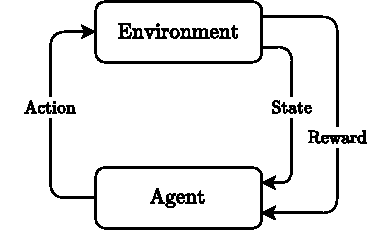
\includegraphics[width=8cm]{agent-enviroment-2}
  
  \caption{\label{fig:agent-enviroment} The agent-environment interface}
\end{figure}
% stateDiagram-v2
%     direction LR
%     a : Agent
%     e : Enviroment

%     a --> e : Action
%     e --> a : Reward
%     e --> a : State

The agent comprises the entire decision-making entity in an MDP; anything unknown or not wholly under the agent's control is called the agent's environment. In the context of reinforcement learning, the environment is essentially the dynamics of the MDP. Figure~\ref{fig:agent-enviroment} demonstrates how the agent and environments affect each other in an MDP. 

\label{policy-informal-definition}
For learning agents, we wish to improve the agent's behaviour over time. For this purpose, we introduce a policy $\pi$. This policy defines the action chosen by an agent under a particular state. The policy can be represented with a lookup table like in Q-learning\ref{chap:q-learning} or a more complex process such as deep Q-learning. A policy like this is not hard-coded, allowing the agent to update the policy based on the information the agent learns from the environment. 


\section{Policy and Value functions}

After each action, a reward is received. It follows that the goal of an agent should be to choose the actions to maximise these reward signals received. Following the Markov principle and the definition of an MDP, this reward only depends on the current state and the action chosen. Consequently, being in some states and performing some actions are more valuable to the agent than other states and actions. We can define value functions: 
\begin{itemize}
  \item $v(s)$ function determines the value of being in a given state
  \item $q(s, a)$ function determines the value of being in a given state and performing a specific action
\end{itemize}



\begin{figure}[H]
  \centering
  
  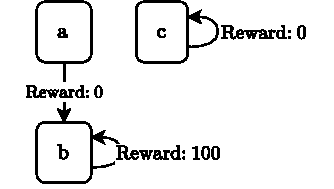
\includegraphics[width=8cm]{reward-example-2}
  
  \caption{\label{fig:reward-example} An example of transitive value of states $v(b) > v(a) > v(c)$}
\end{figure}

Intuitively, the value of being in a state is more than only its immediate reward that might be found from performing actions in that state. It is also related to the potential future reward that might be achieved in the reachable subsequent states. This can be demonstrated with two states $a$, and $b$, where there is a large reward at $b$ and the only way to reach $b$ is through $a$. It is clear that despite the identical immediate rewards, the state $a$ is more valuable than $c$ due to future potential at $b$ available at $a$. However, $a$ can be considered less valuable than $b$, because it always requires more steps to achieve the reward from $a$ than at $b$. To account for our perchance for more immediate rewards, the value function should also discount future value with a parameter $\gamma$. 


These value functions go hand in hand with an agent's policy; a good policy maximises being in valuable states and performing valuable actions. On the other side of the coin, the value is determined by the subsequent states and rewards, which are in part determined by the actions the policy selects. Basing the policy on the value function gives the value function's definition impact over that agent's decision-making, in particular, the discount rate ($\gamma$). With high discount rates $\gamma \approx 1$ the agent can be far-sighted and ignore short-term high-reward actions available to it and take longer to learn. With low discount rates $\gamma \approx 0$, the agent can be short-sighted, ignoring the potential long-term benefits of certain actions.

While the policy is informally described at the end of chapter~\ref{policy-informal-definition}, a formal definition of a policy ($\pi$) is the probability distribution of an agent picking a given action in a given state:

\begin{equation}
  \pi(a \ |\ s) \doteq \Pr(A_t = a | S_t = s)
  \label{eqn:policy-def}
\end{equation}



Where $s \in \mathcal{S}$ and $a \in \mathcal{A}_s$. This definition shows how the policy can be stochastic. A stochastic policy can be beneficial in many ways, such as breaking ties where multiple actions are equally good and choosing between when to explore more or seek rewards. 

\subsection{optimal policy/value function via the Bellman equation}

With a known policy and dynamics, the future state can be wholly determined, allowing for a complete mathematical definition of the value functions under a given policy that describes our above intuitions. for the state-value function ($v$) and action-value function ($q$) under a policy $\pi$ we have the formulas:


\begin{align}
  q_\pi(s,a) & \doteq \sum_{s',r}p(s',r\ |\ s, a)[r + \gamma v_\pi(s')]\label{eqn:q-def} \\
  v_\pi(s)   & \doteq \sum_a \pi(a\ |\ s) q_\pi(s,a) \label{eqn:v-def}
\end{align}

These value functions are defined recursively in terms of each other; these definitions can be unrolled to only be in terms of themselves. The unrolled form of the state-value function is known as the Bellman equation. These equations are named Richard Bellman, who, in the process of developing the field of dynamic programming, created them\cite{bellman1957}.   

These functions demonstrate the intertwined relationships between the policy chosen and the value of that state if there is a particularly valuable action $a^\ast$ such that $q_\pi(s,a^\ast)$ is far better than for all other actions. A policy $\pi(a^\ast\ |\ s) = 0$ would hamper the potential value of $s$. Therefore, the value function can be used to compare how well different policies perform. If for policy $\pi_a$ there does not exist another policy $\pi_b$ such that $\pi_b$ has a better value $v_{\pi_b}(s) > v_{\pi_a}(s)$ for all states $s \in \mathcal{S}$ then we can consider this policy $\pi_a$ an optimal policy. There may be many optimal policies; however, we often do not need to distinguish them, so we often denote any optimal policy with $\pi_\ast$. This is because all optimal policies share the same state-value, and by definition action-value, function, we denote this $ v_\ast$ and $q_\ast$. The optimal value function $v_\ast$ is known as the Bellman optimality equation. These optimal equations can be written formally as:


\begin{align}
  q_\ast(s,a) & \doteq \max_\pi q_\pi(s,a)\label{eqn:q-optimal-def} \\
  v_\ast(s)   & \doteq \max_\pi v_\pi(s) \label{eqn:v-optimal-def}
\end{align}




\subsection{Finding optimal policies by iteration}\label{iteration-approaches}

Although optimal policies exist, finding them is another matter. The policy search space is potentially infinite so an intelligent method is required. An optimal policy can be extracted from an optimal value function and the dynamics of the MDP; the optimal policy would only select actions that result in the highest value. Finding the optimal value function with the optimal policy is straightforward, but this is a catch-22. The optimal value function must be self-consistent with the Bellman equations. One approach to solving these equations is iteration, for each step moving slightly closer to the optimal solution from an initial guess. 

\subsubsection{Policy Iteration}

In policy iteration, we improve a policy over time until it is optimal. updating a policy like this is only possible because of the policy improvement theorem. This theorem considers if we have a policy $\pi_{\text{old}}$. We are at some state $s$, $\pi_{\text{old}}$ will pick the action $a$ under this state $\pi_{\text{old}}(a\ |\ s) = 1$ what happens if we consider some other action $a'$ but then continue to follow the original policy. Because we continue to follow the original policy, we can use the existing value function $v_{\pi_{\text{old}}}(S_{t+1})$ for the subsequent states. We call this slightly adjusted policy $\pi_{\text{new}}$. By applying the Bellman equations and the existing value function then we can recalculate the value at $s$ of $\pi_{\text{new}}$ if this new value is better than the original policy then we know that $\pi_{\text{new}}$ must be as good if not better for all states $s \in \mathcal{S}$ than $\pi_{\text{old}}$ thus $\pi_{\text{new}}$ would be a better policy. 


\begin{equation}
  \sum_a \pi_{\text{new}}(a\ |\ s) q_{\pi_{\text{old}}}(s,a) \ge v_{\pi_{\text{old}}}(s) \Rightarrow  \pi_{\text{new}} \ge \pi_{\text{old}}
  \label{eqn:policy-improvement-theorem}
\end{equation}

For some policy $\pi$ you can apply this policy improvement theorem for every state and action in the MDP. This approach of comparing all actions over all states is called policy improvement. This policy improvement step can be applied iteratively until the policy stops improving. If the policy does not improve over this policy improvement step, then all of the actions are optimal, and this policy is optimal

Although this policy improvement sounds computationally expensive, each state can be considered simultaneously and with a shared base policy; in each iteration, the state-value function is the same; caching this removes redundant calculations. Calculating the value function is improved by using an iterative approach and utilising the previous value function as a launching point.  


\subsubsection{Value Iteration}

Policy iteration is a practical approach, for a finite MDP is guaranteed to finish in finite time. In practice, policy improvement does better and only takes a few iterations. However, in each iteration, multiple full sweeps of the state space are required. The idea of value iteration is to improve the policy within the value iteration step. This value iteration approach only requires one iteration. 

The Bellman equation\ref{eqn:v-def} can be used as an update rule to compute the value function iteratively. A table of values is maintained for each state, initialised randomly. The value of each state can be updated based on the immediate reward and the current estimates of the subsequent states; this is guaranteed to reduce the error at that state because the $\gamma$ discount rate discounts the error at the subsequent state. This process is called bootstrapping; the smaller $\gamma$, the quicker the error rate will decrease, and the faster the process will converge. When the inconsistency at each state is suitable, the process will stop. 

This standard approach uses the traditional value Bellman equation\ref{eqn:v-def} to find the value for a given policy. In value iteration, the policy is one that exclusively picks the action that has the maximum value. This policy is optimal for the optimal value function; when the value iteration converges, it must be optimal because of these conditions. This augmented update rule can be defined as:

\begin{align}
  q_{\text{max}}(s,a)          & \doteq \sum_{s',r}p(s',r\ |\ s, a)[r + \gamma v_{\text{max}}(s')] \tag{from \ref{eqn:q-def}} \\
  v_{\text{max}}(s)            & \leftarrow  \max_a q_{\text{max}}(s,a) \label{eqn:v-update}                                  \\
  \therefore v_{\text{max}}(s) & \leftarrow  \max_a \sum_{s',r}p(s',r\ |\ s, a)[r + \gamma v_{\text{max}}(s')]
\end{align}


As this new update rule involves no explicit policy, a final step is required in value iteration to extract an explicit policy. In this step, the action that leads to the best value for each step, according to the $q_\ast$ function.$q_\ast$, can be derived from the $v_\ast$ with the dynamics $p$ function.


\section{Learning as incrementally optimising policy in a MDP}

Learning is the process of acquiring new information and skills. There are many different ways organisms can learn, In psychology one of the methods is called Operant Conditioning. In Operant Conditioning the learner receives feedback from the environment as either a reward or punishment for completing different actions\cite{staddon2003operant}. In an experiment this could be some food for opening a door, this feedback influences the learner's future actions. This is an equivalent mechanism that reinforcement learning operates under. It is, for this reason, that RL is considered the dominant theoretical framework for operant learning \cite{shteingart2014reinforcement}. 

To demonstrate learning as policy optimisation consider an agent that is introduced to a new Markov environment. This agent has no prior knowledge therefore its initial policy is independent of the environment's features. eventually, the agent will pick some action in a state and receive some reward from the environment. This information can be used to update the policy to prioritise that one successful action. since the environment obeys the Markov property repeating this successful action will continue to reward. If the agent continues to optimise its policy as it finds rewards then it can improve its average reward. through incrementally optimising its policy this agent has learnt what are the successful actions and improved its behaviour.



\section{Q-learning}\label{chap:q-learning}


Q-learning is like value and policy iteration; all search for an optimal value function. However, Q-learning operates under extra constraints. The value and policy iteration extensively use the MDP's dynamics ($p$). In most real-world problems, the dynamics are unknown or too complex to be represented accurately. Iteration approaches can be adapted using samples to work without $p$. Samples are captured from the environment when the agent performs actions, which can be chosen randomly or by following another policy. Monti-Carlo is another technique that uses samples to emulate the value functions more directly, but these approaches are inherently offline. While offline methods have many advantages, their shortcomings, such as the inability to adapt to changing environments, make them unsuitable for many applications. 

\subsection{Temporal difference}

Temporal difference (TD) algorithms are another class of RL algorithms. TD is an online process that improves the policy as new data becomes available. The goal of TD is to minimise the $\delta$ parameter that represents the difference (error) between the observed and predicted rewards. This difference $\delta$ is used to update the model like the iterative approaches we bootstrap our model over time. The magnitude of each update is controlled with the learning rate parameter, $\alpha$. $\alpha$ helps avoid overfitting to samples since observations made in the real world may be noisy and change over time. The learning rate and discount rate can affect the convergence rate for TD; however, these are distinct variables and have different purposes. When $\alpha$ is low, the process will take longer to converge; however, if $\alpha$ is too large, the process may diverge

Reinforcement learning algorithms typically can learn in two fashions: on-policy and off-policy. On-policy algorithms learn while the agent uses the policy being improved; an example is SARSA. Off-policy algorithms typically learn the value functions while the agent follows a different \say{behaviour} policy. While on-policy techniques can start exploiting their knowledge for reward quickly, they can get stuck in local minima. Off-policy techniques can provide more control over the exploration and exploitation. Q-learning is an off-policy TD reinforcement learning algorithm implemented in this project.

\subsection{Definition}

As the name suggests, Q-learning learns the optimal action-value function $q$ to find the optimal policy. TD techniques must learn the $q$ function directly. The $v$ function requires knowledge of the dynamics to derive the optimal policy; however, with the $q$ alone, the optimal policy can be determined. For this purpose, Q-learning needs to maintain a table entry for each action in each state so these entries can be updated after each observed action. We will represent this estimate of $q$ with $Q$. There are five parts to each transition: 
\begin{itemize}
  \item $S_{t-1}$ the previous state before the transition
  \item $A_{t-1}$ the action that was performed
  \item $R_t$ the reward received
  \item $S_t$ the new and now current state
\end{itemize}

Q-learning uses these observations to update its estimates with this formula:

\begin{equation}
  Q(S_{t-1}, A_{t-1}) \leftarrow Q(S_{t-1}, A_{t-1}) +  \alpha [R_t + \gamma \max_a(Q(S_t,a)) - Q(S_{t-1}, A_{t-1})]
  \label{eqn:q-learning-update-formula}
\end{equation}


This formula can be thought of as interpolating the old estimate at the old state $Q(S_{t-1}, A_{t-1})$ with this new observed Q-value $R_t + \gamma \max_a(Q(S_t, a))$. When $\alpha = 1$, this formula replaces the existing value with the new observed Q-value.  When $\alpha = 0$, the observation is ignored like it never happened. The formula $R_t + \gamma \max_a(Q(S_t, a))$ calculates the new observed Q-value based upon the same principle as value iteration; the implicit policy is to pick the best possible action. 

\subsection{Implementation conditions}\label{sect:impl-conditions}

Q-learning is guaranteed to eventually converge the $Q$ estimates to the optimal q values $q_\ast$ provided the behaviour function visits all state-action pairs infinitely often. In practice, these q-values do not need to be perfect to derive an optimal policy. However, it can still take many visits to converge enough. Many observations may be necessary to build up a picture of the probability distribution and isolate noise. However, another reason for repeated observations is that the behaviour policy moves the agent forward in time, but the Q-learning table updates the last state. This conflicts as information propagates in the opposite direction of the updates that spread it. For example, suppose a sequence of $n$ states-actions have no reward but lead to some large reward at the end. as the behaviour completes these actions. In that case, only the last action will be updated to reflect the potential value, and every time the sequence is repeated, some of the value will propagate back one step. Many Q-learning implementations like ours will replay recent observations in reverse order to improve this performance. This is called the action-replay process (ARP). Replaying observations can be particularly effective when getting new observations is costly or slow, allowing for quicker convergence.


In \ref{eqn:q-learning-update-formula}, we can see how $\alpha$ controls the influence of each observation. But how do we tune this hyper-parameter? One option is to treat it like other hyperparameters where possible and use previous experimentation to find a practical value. However, one of the main reasons to use RL is that it does not require prior knowledge, so this is not always suitable. A fixed learning rate may not also be suitable. Some observations may be more important than others; It has been observed that a decaying learning rate has been more effective. It is believed that a decaying learning rate allows for learning algorithms to avoid local minima at the beginning with the large learning rate and then settle on a global minima as the learning rate decays\cite{decayingLearningRates}. The paper \say{Learning Rates for Q-learning}\cite{even2003learning} derives how polynomial learning rates such as $\alpha = 1/t^\omega$ converge much better than linear ($\alpha = 1/t$) rates.

Picking the behavioural policy is important; it must balance exploring and gaining rewards (exploitation). For some policies, the $\varepsilon$ parameter determines the ratio of exploration and exploitation, a high $\varepsilon$ would result in more exploration. There are two common behaviour policies for this:
\begin{itemize}
  \item $\varepsilon$-greedy: this policy randomly picks between (A) selecting the best action based on the current Q-table or (B) selecting another action. A or B is random with the ratio determined by $\varepsilon$
  \item $\varepsilon$-soft: this policy assigns probabilities to all actions based upon their q-values, biased towards the higher Q-values by $\varepsilon$. Then, random actions are chosen according to this probability distribution.
\end{itemize}

Both $\varepsilon$-greedy and $\varepsilon$-soft policies utilise the current $Q$ value estimates, which can lead to bias. Incorrect over-optimistic and over-pessimistic estimates can lead to a poor distribution of observations, compounding these effects. One approach to limit bias is called double Q-learning. This is where two Q-learning tables are kept, and actions are chosen based upon alternating tables this helps average out the bias and improves the accuracy of estimates.

\chapter{Exploration Strategy Effectiveness}

Q-learning is an off-policy process, which means that the policy that the policy that it is learning and improving is not necessarily the same as the policy it is following during exploration. By this, the actions chosen by a Q-learning agent may be independent of its current beliefs of the values of each action. Off-policy learning has several advantages, it may explore more fairly and completely than an on-policy approach. An on-policy approach may be incentivised to explore thoroughly if its initial estimates are particularly optimistic. However, in a stochastic environment where rewards are random with a large degree of spread, it may still be difficult for an on-policy technique to properly assess the rewards before falling into an in-optimal pattern.  

On-policy reinforcement learning algorithms such as SARSA do have many advantages in deep reinforcement learning (DRL). In DRL a deep artificial neural network is used to estimate the Q-values\cite{deepRLOverview}. DRL can help generalise reinforcement learning to larger state spaces than is possible with tabular methods. Typically in this context, fully off-policy methods do not perform as well as on-policy or hybrid methods \cite{deepOnVsOffPolicy}. since off-policy methods suffer from instability.

In this project, I have focused on the off-policy Q-learning method. This chapter details the performance and effects of different exploration strategies. An exploration strategy is the policy that the agent follows during training as opposed to the learnt policy. This exploration strategy may be any method to select an action, however, to maintain the guarantees of convergence this policy must reach all states infinitely often (\ref{sect:impl-conditions}). While a random action section, a random walk, does meet the convergence criteria it is not efficient in terms of rewards received or information gained. As an improvement in these measures, more sophisticated strategies have been developed that take into account many factors.

To assess the effectiveness of exploration strategies the optimal policy sets a benchmark that there are two main measures. The first measure is called regret, it is the difference in cumulative reward between an optimal agent and the exploitation strategy during learning. The second measure is called best policy identification (BPI) this relates to the number of samples taken to identify a nearly optimal policy\cite{modelFree}. Reducing the BPI will in general reduce the regret. I believe with a suitably large time horizon, that the effects of reducing regret will correspond to a reduction in BPI since the benefits of an optimal policy will eventually pay off the costs associated with finding it. For consistency, this project will focus on regret minimisation.


\section{TODO - \texorpdfstring{$\varepsilon$}{Lg}-Greedy}

The $\varepsilon$-Greedy is the most straightforward strategy implemented in this project and it acts as a good baseline. In its basic form, there is a parameter $\varepsilon$ that controls the probability of the agent acting in two modes. The first and typically most common mode is where the agent selects the best action based on the current Q-estimates. In this first mode, the agent is essentially operating in an on-policy manner. In the second mode, the agent selects an action at random \ref{sect:impl-conditions}.

This epsilon parameter controls the ratio between the agent's exploration and exploitation. Having high exploitation can garner more rewards in the short term but this has a large opportunity cost of not finding potentially lucrative strategies. On the other hand, if you are already following an optimal policy an exploratory action would not be optimal, and in the case of the cliff environment, it can be potentially devastating. In the beginning, higher exploration may be necessary to avoid local minima, but once the policy has started to converge higher exploitation can be more rewarding. To address this issue the $\varepsilon$ parameter can be dynamically adjusted during training. This project implements the traditional discounting with a fixed hyperparameter however more advanced reward-based techniques have been found more successful\cite{rewardEpsilonDecay}.

\section{TODO - Upper Confidence Bound}

The upper confidence bound (UCB) exploration strategy uses the current Q value estimates to direct its decisions however instead of using randomness to dictate exploration, it uses an informed method. UCB prioritises actions that have the highest potential for reward. The potential of value is determined from two factors the current value estimate and a measure of confidence in the value estimate. The key idea behind this confidence measure is that it relates to the number of samples that have been made of the state action\cite{sutton2018reinforcement}. This relationship is defined in the following rule:


\begin{equation}
  A_t \doteq \underset{a}{\operatorname{argmax}}\left [Q_t(a)+ c\sqrt{\frac{\ln t}{N_t(a)}} \ \right ]
  \label{eqn:ucb}
\end{equation}
\cite{sutton2018reinforcement}

where $A_t$ represents the action chosen at time $t$, and $N_t(a)$ represents the number of samples of action $a$ have been taken at the current time. 


In essence, this equation is optimistic as it will never underestimate or explore an action. It also provides a natural balance between exploration and exploitation, Without a discount factor this strategy naturally tapers off exploration over time. Furthermore instead of even exploration like $\varepsilon$-Greedy; UCB avoids redundant exploration in areas that have already been covered. However, UCB is not without hyper-parameters. $c$ controls the exploration balance; higher values encourage more exploration.

\section{TODO - Model-Free Best Policy Identification}

Model-Free Best Policy Identification (MF-BPI) is a state-of-the-art method that has demonstrated an improvement in exploration over its contemporaries such as UCB \cite{modelFree}. This exploration strategy uses an allocation vector $\omega$ that distributes the search effort across the state-action space. The MF-BPI algorithms aim to optimise this allocation vector for the BPI metric. To handle the uncertainty in the estimates MF-BPI maintains an ensemble of value tables to measure their variance. MF-BPI also uses a bootstrapping technique to ensure that the uncertainty decreases over time. Due to this bootstrapping, they claim that MF-BPI does not require forced exploration to ensure all state-action pairs are visited infinitely often however their implementations provided did include forced exploration.


\section{Hyperparameter Selection}

\begin{figure}[H]
  \centering
  
  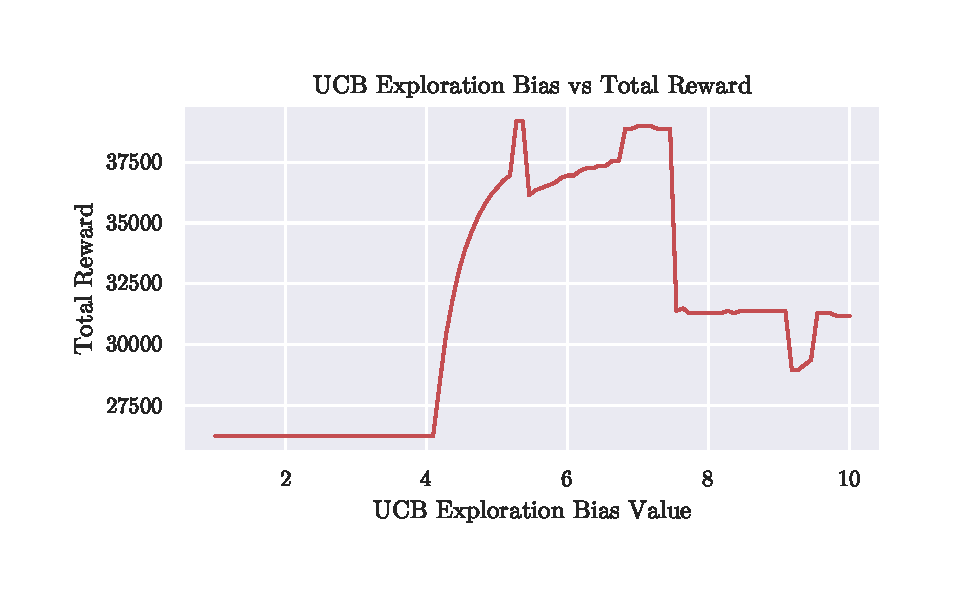
\includegraphics[trim={0 1cm 0 1cm},clip,width=\textwidth]{hyper-paramiters/ucb-exploration}
  
  \caption{\label{fig:ucb-exploration-bias}}
\end{figure}

Q-learning itself and each exploration strategy require some parameters which are set outside of the learning process. Figure~\ref{fig:ucb-exploration-bias} Demonstrates how hyper-parameter values can have a profound impact on the effectiveness of the agent. However, selecting the best parameters is not straightforward. The first difficulty is that the best parameter choice depends on the agent and the environment that it operates on so they are not transferable and must be found through experimentation. The second difficulty is that the hyper-parameters are not independent different choices may compound or interfere with each other.  Finally building on the second issue is the number of parameters, for Q-learning with $\varepsilon$-greedy there are 6 tunable parameters, This makes visualising the whole hyper-parameter space impossible. 


For this reason, the application contains multiple systems for finding the appropriate values for these hyper-parameters. Firstly the hyper-parameters are configurable in the application's main configuration file. This configuration drives the parameters used by the main simulation and the defaults used in the report system. The hyper-parameter report system runs multiple simulations in the background and collates their results. This system allows the user to visualise and compare the effects of varying each parameter individually. 


This report system overcomes the dimensionality visualisation issue by displaying a single axis-aligned slice of the space at a time. This approach is great for isolating the effects of a single parameter and fine-tuning parameters. Unfortunately, this approach cannot display the effects of any parameter combinations that do not coincide along one of the hyperparameter axes. Due to this limitation, the visualisations may display a local minimum and completely miss a global minimum. 

A hyper-parameter search system is implemented to find the best baseline for fair comparisons. There are a few popular search strategies for hyperparameter optimization such as grid search, random search, and genetic algorithms \cite{searchStrategies}. Grid-search is a very popular approach for its advantages such as simplicity, uniformity and parallelisation \cite{searchStrategies}. however, it suffers from the curse of dimensionality\cite{searchStrategies} so it was not suitable for this application. Instead, the random search strategy has been implemented. This strategy is highly amenable to parallelisation, A number of workers are used and they pick the parameters at random and run simulations independently. In this manner, the random search strategy does not require orchestration of the parameters and is resumable, synchronisation is only necessary when collating results to avoid race conditions.


Since the performance is highly dependent on the environment; the same cliff dynamics have been used in all the graphs provided in this chapter. Furthermore, all of the episodes are equal in length so the cumulative reward achieved is comparable. An agent that directly follows the optimal policy without learning can achieve a cumulative reward of 45500 under the same conditions. This provides the upper bound on the agent's performance and the bar from which to determine regret. In the following sections, a Q-learning agent with the $\varepsilon$-greedy exploitation strategy is used for the evaluation. This strategy is stochastic and its variability affects the performance. To account for this influence many simulations are run for each configuration. Each graph plots the mean reward in red and a 95\% confidence interval in blue. The following sections will cover an interesting subset of the hyper-parameters and discuss my findings.


\subsection{Initial Optimism}

\begin{figure}[H]
  \centering
  
  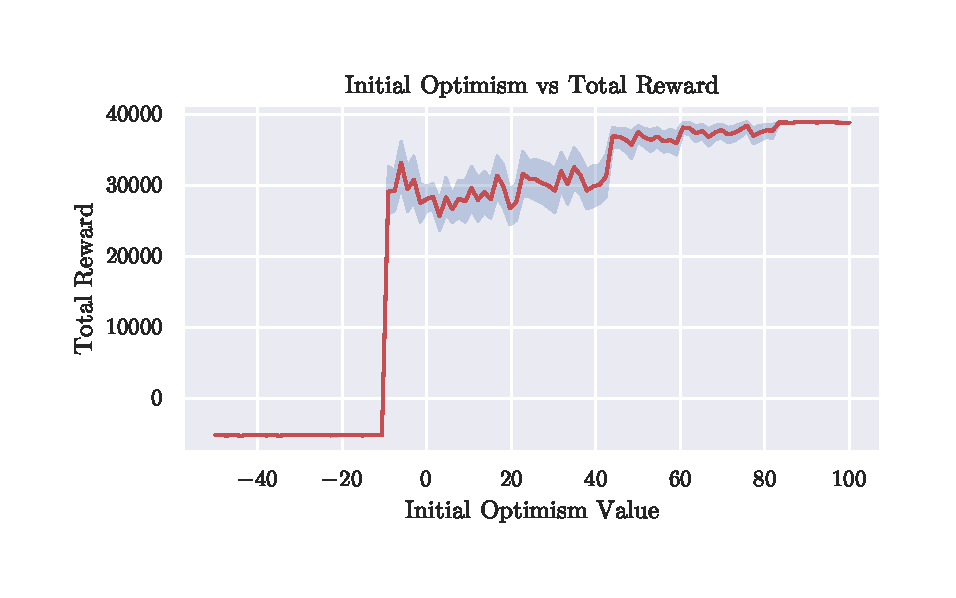
\includegraphics[trim={0 1cm 0 1cm},clip, width=\textwidth]{hyper-paramiters/inital-optimism}
  
  \caption{\label{fig:inital-optimism}}
\end{figure}


The initial optimism hyper-parameter determines the initial Q-value estimates. In essence, this is the agent's interpretation of the value of state actions before the agent has gained any experience of that state action. Since Q-learning is a bootstrapping method depending on parameters such as the learning rate, the discount factor and the rewards provided initial biases may persist through more or less updates. This can be an opportunity to provide information a-priori, value tables from previous agents can provide a head-start \cite{deathTransfer}. While realistic initial estimates are beneficial, figure~\ref{fig:inital-optimism} shows how excessive values can be cost performance. 

When the initial estimate is larger than the actual value of each state this is optimistic. Optimism encourages the agent to try unknown states over known states since the optimistic initial values will be strictly better than the more realistic derived value. On the other hand, pessimistic values act oppositely, discouraging exploration as known states seem better than unknown states. You can see this demonstrated in figure~\ref{fig:inital-optimism}, in the pessimistic region (left of 100) the variability is higher because the agent relies entirely on the random forced exploration. 

Increasing optimism gradually decreases performance as the agent over-explores and neglects exploitation. The effect is similar for pessimism however the performance hits a cliff after the initial estimates become negative. At this point, the agent gets stuck repeatedly choosing the same state or states. I believe this may be a consequence of several factors. Firstly the other parameters aren't configured for this degree of pessimism, so the agent can't reach the goal based on forced exploration alone, and the pessimism stops it from exploring enough to find it. Secondly, the discount factor works in reverse when all values are negative it encourages taking longer. Finally, Q-learning's maximisation bias may be inhibiting its ability to propagate these negative updates correctly \cite{doubleQLearning}\cite{sutton2018reinforcement}. 


\subsection{Learning Rate \texorpdfstring{$\alpha$}{Lg}}

\begin{figure}[H]
  \centering
  
  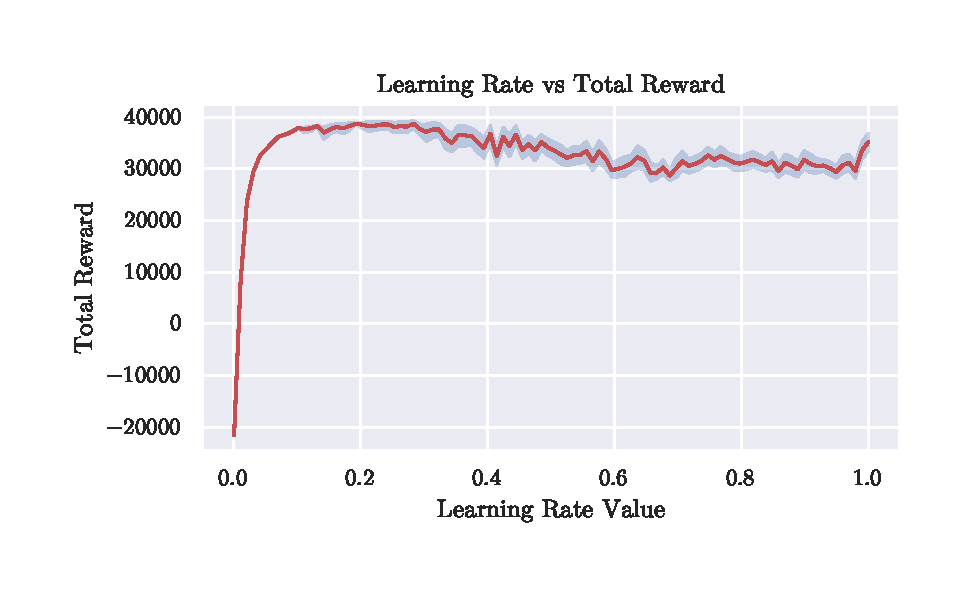
\includegraphics[trim={0 1cm 0 1cm},clip,width=\textwidth]{hyper-paramiters/learning-rate}
  
  \caption{\label{fig:learning-rate}}
\end{figure}

The learning rate $\alpha$ is another hyperparameter of Q-learning\ref{eqn:q-learning-update-formula}. This parameter controls how much each new TD estimate will update the current estimates. For stochastic environments getting this value right is crucial, If set too high the variability from the individual observations could lead to instability and the Q-table may not even converge at all. The cliff dynamics that are used in this demonstration are completely deterministic. 
The larger the learning rate the less updates are necessary for the values to converge. However this can be a double edged sword because in the current configuration optimistic initial estimates drive the majority of the exploration. Therefore more smaller updates encourage more thorough but slower exploration whereas larger updates are more rapid but unstable exploration.


Figure~\ref {fig:learning-rate} shows the balance of learning rate and how this impacts performance. In the range $0.2$ to $1$ there is a plateau where the stability and speed of convergence are in balance. However as the learning rate approaches zero the performance diminishes rapidly as the time taken to learn anything extends. In this region the exploration period inhibits the agent's ability to exploit the environment.

\subsection{TODO - \texorpdfstring{$\varepsilon$}{Lg}-Greedy Decay Rate}

\begin{figure}[H]
  \centering
  
  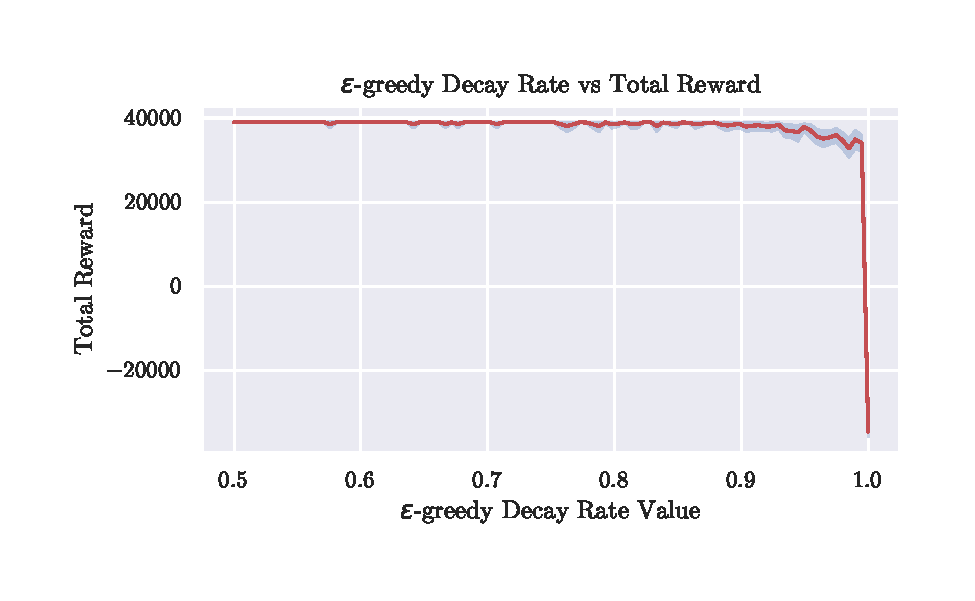
\includegraphics[trim={0 1cm 0 1cm},clip,width=\textwidth]{hyper-paramiters/epsilon-greedy-decay-full}
  
  \caption{\label{fig:epsilon-greedy-decay-full}Wide range $\varepsilon$-greedy decay rate graph.}
\end{figure}

The $\varepsilon$-greedy decay rate (EGDR) parameter is an important an unique parameter. Figure~\ref{fig:epsilon-greedy-decay-full} demonstrates how just a miniscule amount of decay has a substantial improvement on the agent's regret completely changing the agents performance. Without EGDR the cumulative reward was negative. This follows from how $\varepsilon$-greedy acts in a partially off-policy, in the cliff dynamics the optimal policy is one that minimises the distance travelled and therefore travels right next to the cliff face. This becomes problematic when $\varepsilon$-greedy introduces its off-policy exploration actions, which randomly cause the agent to select the action to jump off the cliff incurring a large penalty.

An on-policy method may account for the chance of selecting exploratory actions in its value estimates encouraging the agent to give the cliff a wide berth or choose to limit the exploratory actions. another approach is to reduce the exploration rate once the agent has had the opportunity to learn. This application has implemented exponential decay for the exploration ratio $\varepsilon$. This exponential decay is controlled via two hyperparameter the initial value and the decay rate. In this procedure the exploration ratio $\varepsilon$ can be computed as: 

\begin{equation}
  \varepsilon_t = \lambda^t \cdot \varepsilon_0
\end{equation}

Where $\varepsilon_t$ is the exploration ratio at the time step $t$ and $\lambda$ represents the EGDR.

% \begin{figure}[H]
%   \centering
  
%   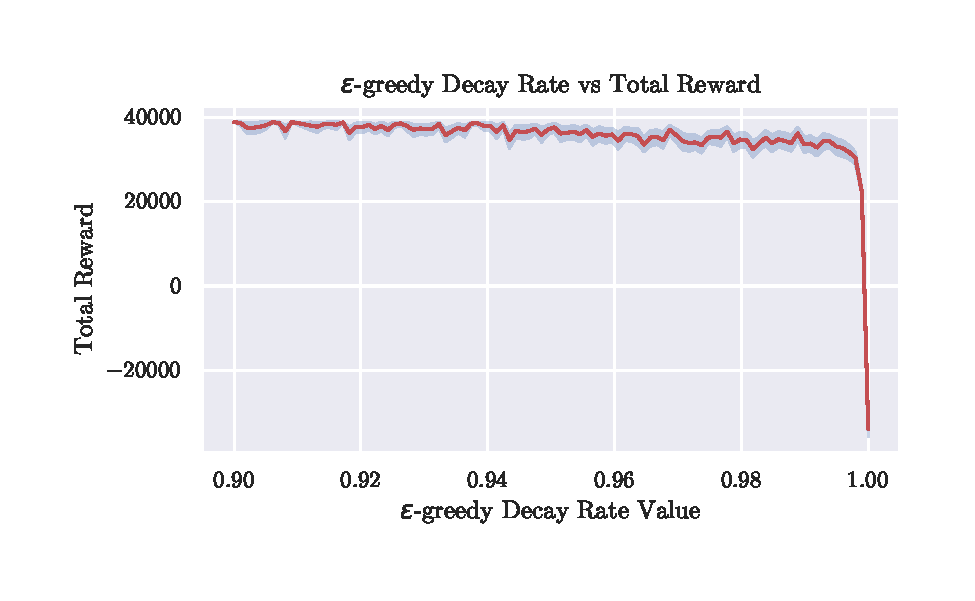
\includegraphics[trim={0 1cm 0 1cm},clip, width=\textwidth]{hyper-paramiters/epsilon-greedy-decay-top-half}
  
%   \caption{\label{fig:epsilon-greedy-decay-zoomed}Narrow range $\varepsilon$-greedy decay rate graph.}
% \end{figure}

\begin{figure}[H]
  \centering
  
  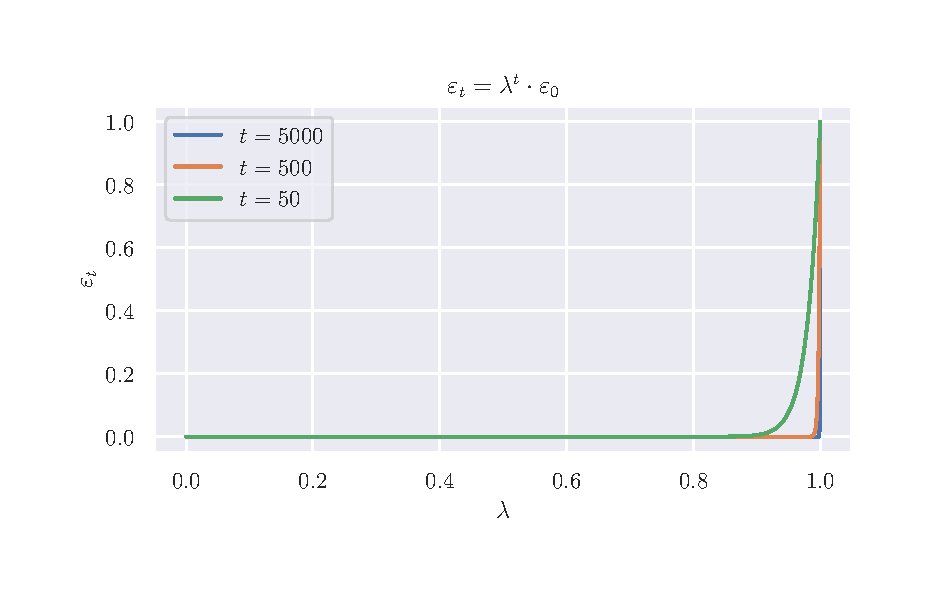
\includegraphics[trim={0 1cm 0 1cm},clip, width=\textwidth]{hyper-paramiters/example-curve.pdf}
  
  \caption{\label{fig:example-curve}}
\end{figure}


EGDR has a very striking form as there is almost no variability in performance until approximately $>0.99$ where the performance almost immediately. This sharp corner follows from EGDR's compounding effects with respect to the time-step and the number of time-steps. Each simulation has 5000 time-steps, figure~\ref{fig:example-curve} demonstrates how with this number of time steps all but the most extreme values will not be reduced to near zero. The figure~\ref{fig:example-curve} also shows how the EGDR parameter can control how long the agent has foced exploration, on this graph a decay rate of $\lambda = 0.99$ would have a 0.6 exploration probability by timestep 50 whereas $\lambda < 0.6$ would have a probability if less than $1 \cdot 10^{-12}$ in other words the figure~\ref{fig:example-curve} shows that depending on the EGDR the exploration phase may take more or less than 50 time-steps. I derive this formula to predict the length of exploration:

\begin{align}
  t_{\text{exploration}} &= \log_{\lambda}(\frac{\varepsilon_{\text{min}}}{\varepsilon_0}) \\
  \varepsilon_{\text{min}} &= 1 - (1-\alpha)^{\frac{1}{d}} \label{eqn:compound-adjustment} 
\end{align}

Where $\varepsilon_{\text{min}}$ is the minimum minimum chance of exploration to consider the agent is still exploring in each time step. This probability also compounds so you can use the equation~\ref{eqn:compound-adjustment} to compensate for the remaining duration of the episode, where $\alpha$ is probability of an exploratory action in the duration $d$ (number of time-steps). 



\subsection{TODO - Discount Rate \texorpdfstring{$\gamma$}{Lg}}

\begin{figure}[H]
  \centering
  
  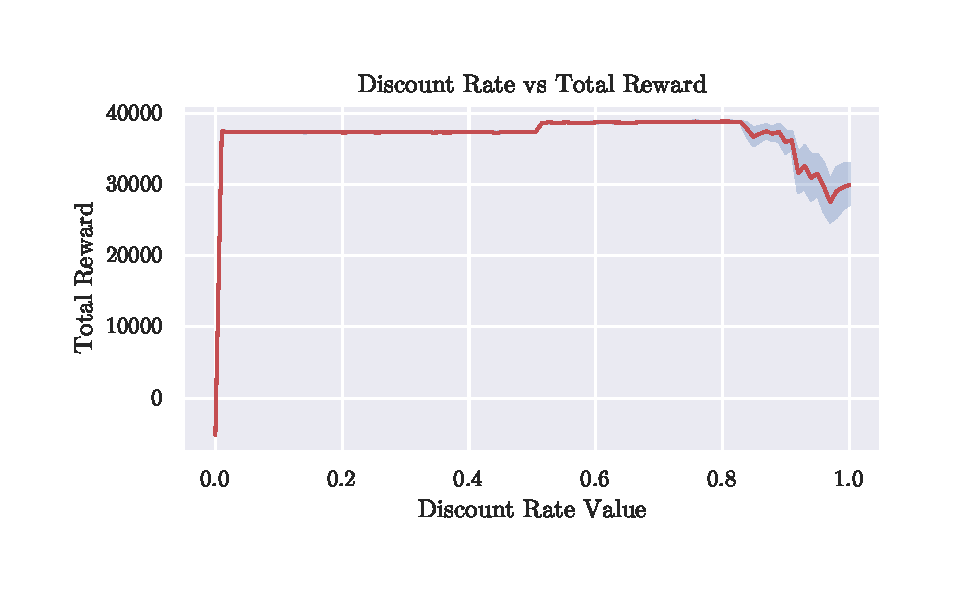
\includegraphics[trim={0 1cm 0 1cm},clip,width=\textwidth]{hyper-paramiters/discount-rate-full}
  
  \caption{\label{fig:discount-rate-full}Full range discount rate graph.}
\end{figure}

\begin{figure}[H]
  \centering
  
  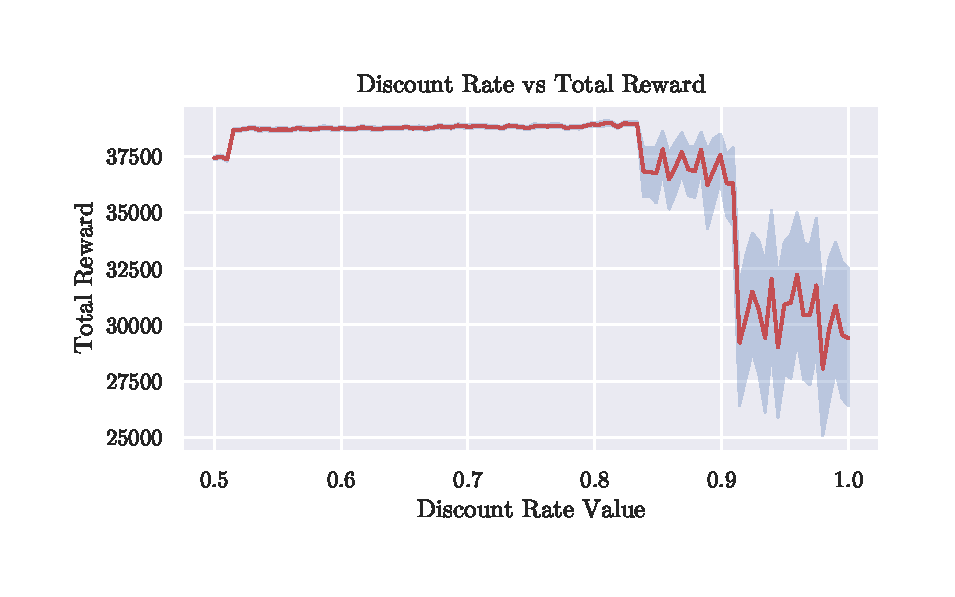
\includegraphics[trim={0 1cm 0 1cm},clip,width=\textwidth]{hyper-paramiters/discount-rate-top-half}
  
  \caption{\label{fig:discount-rate-zoomed}Reduced range discount rate graph.}
\end{figure}



\section{TODO - Conclusions}

\chapter{TODO - Project Analysis}

Critical analysis and Discussion (10\%): A discussion of actual project achievements and how successful the project was. Clear evidence of reflection on the project process, its difficulties, successes and future enhancements. Any conclusions or results analysed or discussed appropriately;


%%%% ADD YOUR BIBLIOGRAPHY HERE
\newpage

\bibliographystyle{IEEEtran}
\bibliography{refrences}
\addcontentsline{toc}{chapter}{Bibliography}

\appendix

\chapter{Diary}





\hypertarget{week-01-180923}{%
  \subsubsection{Week 01 (18/09/23)}\label{week-01-180923}}

\begin{itemize}
  \tightlist
  \item
        (Tue 19) Attended first lecture
  \item
        (Thu 21) Started reading Reinforcement Learning in 'Machine Learning'
        by Tom Mitchell
  \item
        (Fri 22) Finished reading Reinforcement Learning in 'Machine Learning'
        by Tom Mitchell
\end{itemize}

\hypertarget{week-02-250923}{%
  \subsubsection{Week 02 (25/09/23)}\label{week-02-250923}}

\begin{itemize}
  \tightlist
  \item
        (Mon 25) Decided on project idea

        \begin{itemize}
          \tightlist
          \item
                Started draft project plan
          \item
                Abstract
          \item
                Risks
        \end{itemize}
  \item
        (Tue 26) First meeting with Anand

        \begin{itemize}
          \tightlist
          \item
                Started putting together timeline
          \item
                Started reading Reinforcement Learning An Introduction by Richard S.
                Sutton and Andrew G. Barto
        \end{itemize}
  \item
        (Wed 27)

        \begin{itemize}
          \tightlist
          \item
                Attended second lecture
          \item
                moved project plan over to LaTeX
        \end{itemize}
  \item
        (Thu 28) Worked on project plan report

        \begin{itemize}
          \tightlist
          \item
                improved bibliography
        \end{itemize}
\end{itemize}

\hypertarget{week-03-021023}{%
  \subsubsection{Week 03 (02/10/23)}\label{week-03-021023}}

\begin{itemize}
  \tightlist
  \item
        (Tue 03) worked on project plan

        \begin{itemize}
          \tightlist
          \item
                Put together risks section
          \item
                put together timeline
        \end{itemize}
  \item
        (Wed 04) submitted project plan to Anand
  \item
        (Thu 05) Finished project plan

        \begin{itemize}
          \tightlist
          \item
                Improved abstract
          \item
                improved bibliography
        \end{itemize}
\end{itemize}

\hypertarget{week-04-091023}{%
  \subsubsection{Week 04 (09/10/23)}\label{week-04-091023}}

\begin{itemize}
  \tightlist
  \item
        (Wed 11) Gitlab

        \begin{itemize}
          \tightlist
          \item
                Attended lecture about gitlab
          \item
                Moved Code to GitLab

                \begin{itemize}
                  \tightlist
                  \item
                        setup credentials
                  \item
                        updated remotes
                  \item
                        pushed code
                \end{itemize}
        \end{itemize}
  \item
        (Thu 12) Created Initial Interim report from template

        \begin{itemize}
          \tightlist
          \item
                Finished chapter one from Sutton Barto book
        \end{itemize}
\end{itemize}

\hypertarget{week-05-161023}{%
  \subsubsection{Week 05 (16/10/23)}\label{week-05-161023}}

\begin{itemize}
  \tightlist
  \item
        (Mon 16) Continued reading Sutton Barto book

        \begin{itemize}
          \tightlist
          \item
                chapter 2 and some of chapter 3
        \end{itemize}
  \item
        (Wed 18) Continued reading

        \begin{itemize}
          \tightlist
          \item
                finished Chapter 3
          \item
                attended lecture about testing
        \end{itemize}
  \item
        (Thu 19)

        \begin{itemize}
          \tightlist
          \item
                Second Meeting with Anand
        \end{itemize}
  \item
        (Fri 20) Continued reading read subsections on policy improvement
\end{itemize}

\hypertarget{week-06-231023}{%
  \subsubsection{Week 06 (23/10/23)}\label{week-06-231023}}

\begin{itemize}
  \tightlist
  \item
        (Mon 23)

        \begin{itemize}
          \tightlist
          \item
                Continued reading Sutton Barto book

                \begin{itemize}
                  \tightlist
                  \item
                        read chapters 4,6 and skimmed 5
                \end{itemize}
          \item
                Met Anand to discuss my project plan
        \end{itemize}
\end{itemize}

\hypertarget{week-07-301023}{%
  \subsubsection{Week 07 (30/10/23)}\label{week-07-301023}}

\begin{itemize}
  \tightlist
  \item
        (Thu 02)

        \begin{itemize}
          \tightlist
          \item
                Started MDP Report
          \item
                Third Meeting with Anand
        \end{itemize}
  \item
        (Weekend 4-5)

        \begin{itemize}
          \tightlist
          \item
                Completed MDP Report
        \end{itemize}
\end{itemize}

\hypertarget{week-08-061023}{%
  \subsubsection{Week 08 (06/10/23)}\label{week-08-061023}}

\begin{itemize}
  \tightlist
  \item
        (Mon 06) Started report on the policy and value functions
  \item
        (Tue 07) Completed policy and value report
  \item
        (Wed 08)

        \begin{itemize}
          \tightlist
          \item
                Completed policy and value report
          \item
                Started Q-learning report
        \end{itemize}
  \item
        (Thu 09)

        \begin{itemize}
          \tightlist
          \item
                Completed Q-learning report
          \item
                Started code setup
        \end{itemize}
  \item
        (Weekend 10-11) continued setting up code
\end{itemize}

\hypertarget{week-09-131123}{%
  \subsubsection{Week 09 (13/11/23)}\label{week-09-131123}}

\begin{itemize}
  \tightlist
  \item
        (Mon 13)

        \begin{itemize}
          \tightlist
          \item
                Completed code setup
        \end{itemize}
  \item
        (Tue 14)

        \begin{itemize}
          \tightlist
          \item
                Started vertical slice
        \end{itemize}
  \item
        (Wed 15)

        \begin{itemize}
          \tightlist
          \item
                Started writing collection dynamics method
        \end{itemize}
  \item
        (Thu 16)

        \begin{itemize}
          \tightlist
          \item
                Completed collection dynamics
          \item
                Started implementing value iteration
          \item
                Fourth meeting with Anand
        \end{itemize}
  \item
        (Fri 17)

        \begin{itemize}
          \tightlist
          \item
                completed value iteration agent
        \end{itemize}
\end{itemize}

\hypertarget{week-10-201123}{%
  \subsubsection{Week 10 (20/11/23)}\label{week-10-201123}}

\begin{itemize}
  \tightlist
  \item
        (Mon 20)

        \begin{itemize}
          \tightlist
          \item
                Created controllers to tie view and model together.
          \item
                Tried to display grid with canvas approach

                \begin{itemize}
                  \tightlist
                  \item
                        ran into rendering limitations, with many rectangles rectangles
                        kivy started to have issues with rendering the icons.
                \end{itemize}
        \end{itemize}
  \item
        (Tue 21) tried widget based approach

        \begin{itemize}
          \tightlist
          \item
                Tried using kivy's layout widgets to display the grid
          \item
                while the icons were no longer an issue positioning the grid became
                impossible
          \item
                investigated kivy alternatives
        \end{itemize}
  \item
        (Wed 22) Pivoted to using tkinter

        \begin{itemize}
          \tightlist
          \item
                remade exiting UI in tkinter and updated tooling for working with
                tkinter
          \item
                completed grid world display widget
        \end{itemize}
  \item
        (Thu 23)

        \begin{itemize}
          \tightlist
          \item
                Added button that progresses the state over time.
          \item
                Created methods to provide the Q-value information to the view,
                allowing for visualisation.
        \end{itemize}
  \item
        (Fri 24)

        \begin{itemize}
          \tightlist
          \item
                Started adding Q-value visualisation code,
          \item
                Optimised value iteration code with numba
          \item
                Reworked how cells are provided their information
        \end{itemize}
\end{itemize}

\hypertarget{week-11-271123}{%
  \subsubsection{Week 11 (27/11/23)}\label{week-11-271123}}

\begin{itemize}
  \tightlist
  \item
        (Mon 27) Created tooltip to provide state value information and fixed
        origin inconsistency from the move to tkinter.
  \item
        (Tue 28) Completed system for allowing the user to select between
        different types of displays
  \item
        (Wed 29)

        \begin{itemize}
          \tightlist
          \item
                Improved code \texttt{README} and improved usability
          \item
                Implemented the Q-learning agent with
          \item
                Added simultaneous agents to speed up learning
          \item
                Added opening to project report
        \end{itemize}
  \item
        (Thu 30)

        \begin{itemize}
          \tightlist
          \item
                Improved Interim Report
          \item
                Fifth meeting with Anand

                \begin{itemize}
                  \tightlist
                  \item
                        Anand noticed how the simultaneous agents deviated for the
                        literature
                \end{itemize}
        \end{itemize}
  \item
        (Fri 01) Refactor

        \begin{itemize}
          \tightlist
          \item
                Removed the simultaneous agents feature
          \item
                focused on Improving performance in other ways:

                \begin{itemize}
                  \tightlist
                  \item
                        Split MVC across different processes to avoid the GIL
                  \item
                        Improved rendering approach with Pillow no more odd layout and
                        widgets
                \end{itemize}
          \item
                Started making presentation
        \end{itemize}
  \item
        (Sat 02)

        \begin{itemize}
          \tightlist
          \item
                Completed presentation slides
          \item
                Practised presentation
        \end{itemize}
\end{itemize}

\hypertarget{week-12-081223}{%
  \subsection{Week 12 (08/12/23)}\label{week-12-081223}}

\begin{itemize}
  \tightlist
  \item
        (Mon 04)

        \begin{itemize}
          \tightlist
          \item
                Practised presentation
          \item
                Gave presentation
        \end{itemize}
  \item
        (Fri 08)

        \begin{itemize}
          \tightlist
          \item
                Prepared work for Interim submission
        \end{itemize}
\end{itemize}




\label{endpage}



\end{document}

\end{article}
